\section{Results}
\label{sec:results}

\subsection{Classical versus quantum scaling (E1)}
\label{sec:results-e1}

\Cref{fig:e1} shows classical hitting times and quantum search times for the
four synthetic families. The quantum time is the time of peak success
probability, and the interpolation parameter is selected by
\eqref{eq:lower-bound}. The fitted exponents are collected in
\cref{tab:scaling}. Across all $16$ instances the peak success probability is
between $0.84$ and $1.00$, so the reported $T_q$ values are not driven by
low-probability fluctuations.

\begin{figure}[t]
  \centering
  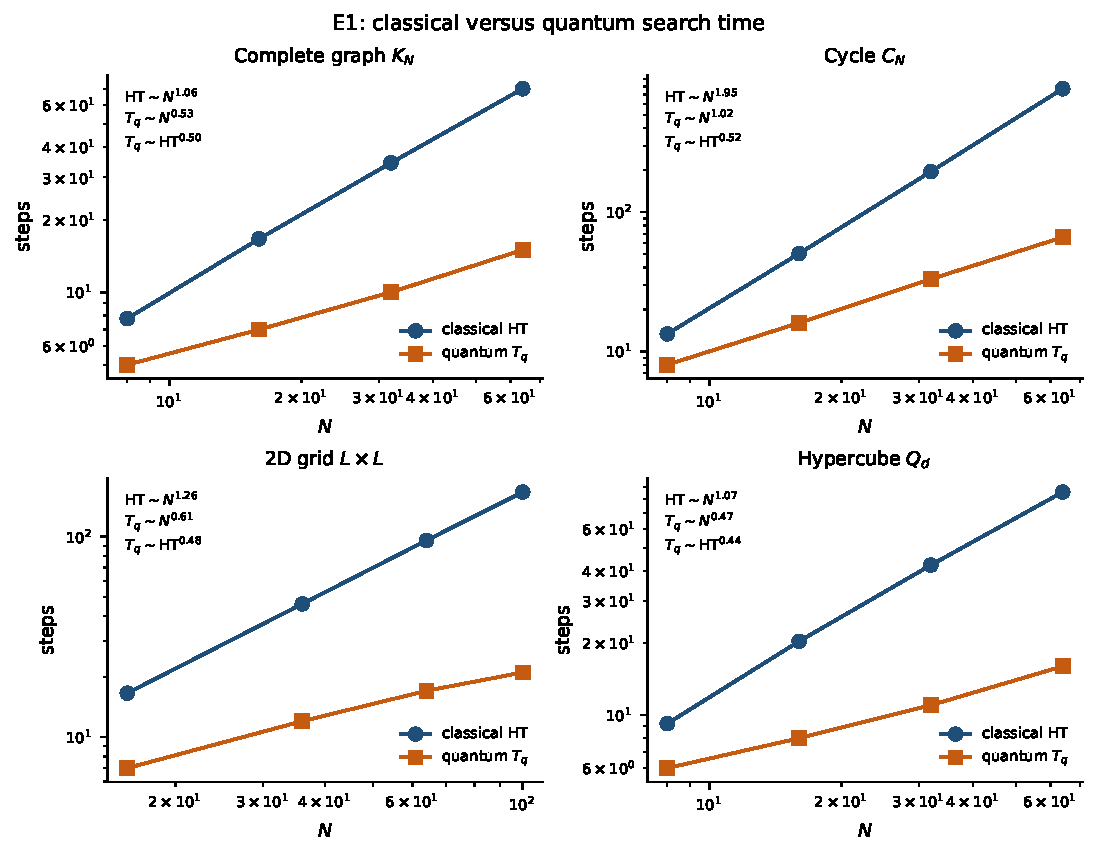
\includegraphics[width=\linewidth]{figures/fig_e1_scaling.pdf}
  \caption{Classical hitting time and quantum search time versus graph size for
  complete graphs, cycles, 2D grids, and hypercubes. Both axes are logarithmic;
  lines are power-law fits. The quantum time tracks a square-root law in the
  classical hitting time rather than in the raw vertex count.}
  \label{fig:e1}
\end{figure}

\begin{table}[t]
  \centering
  \small
  \begin{tabular}{@{}lcccc@{}}
    \toprule
    Family & $\HT\sim N^{\alpha}$ & $T_q\sim N^{\beta}$
    & $T_q\sim \HT^{\gamma}$ & max $\HT/T_q$ \\
    \midrule
    Complete $K_N$ & 1.06 & 0.53 & 0.50 & 4.7 \\
    Cycle $C_N$ & 1.95 & 1.02 & 0.52 & 11.7 \\
    2D grid $L\times L$ & 1.26 & 0.61 & 0.48 & 7.9 \\
    Hypercube $Q_d$ & 1.07 & 0.47 & 0.44 & 5.4 \\
    \bottomrule
  \end{tabular}
  \caption{Fitted scaling exponents from E1. The exponent $\gamma$ is the
  relevant comparison for the AGJK guarantee: it is close to $1/2$ in all four
  families.}
  \label{tab:scaling}
\end{table}

The cycle is the clearest illustration: its classical hitting time grows almost
quadratically ($\alpha=1.95$), while the quantum search time grows almost
linearly ($\beta=1.02$), giving a speedup that reaches $11.7\times$ at $N=64$.
The complete graph ($\HT=\Theta(N)$ exactly) and the hypercube both have
nearly linear hitting times over this size range ($\alpha\approx1.06$--$1.07$),
and the quantum exponents are again close to $1/2$. The grid
shows a slightly larger exponent because the finite-size range does not yet
fully separate $N$ from $\log N$; the fit against $\HT$ gives
$\gamma=0.48$, consistent with the predicted square-root law. The hypercube
has the lowest exponent ($\gamma=0.44$); with only four sizes and integer
$T_q\in\{6,8,11,16\}$ this fit is the least precise of the four.

\FloatBarrier
\subsection{Single, independent, and clustered targets (E2)}
\label{sec:results-e2}

\Cref{fig:e2-success} compares success-probability curves for single,
independent, and clustered marked sets. The independent configuration is
consistently the easiest: on the $8\times8$ grid its mean $\HT$ is $34.7$,
versus $95.5$ for a single target and $79.5$ for a cluster of four. The same
pattern is much stronger on the barbell graph, where independent targets reduce
the hitting time from $2558$ to $16.8$ at $n_{\mathrm{each}}=16$. Clustered
targets give only a modest reduction relative to a single target ($\approx3\%$
on the $n=16$ barbell, $\approx17\%$ on the $8\times8$ grid), far less than
independent targets: once the walker reaches the cluster it still has to find
one of its vertices.

\begin{figure}[t]
  \centering
  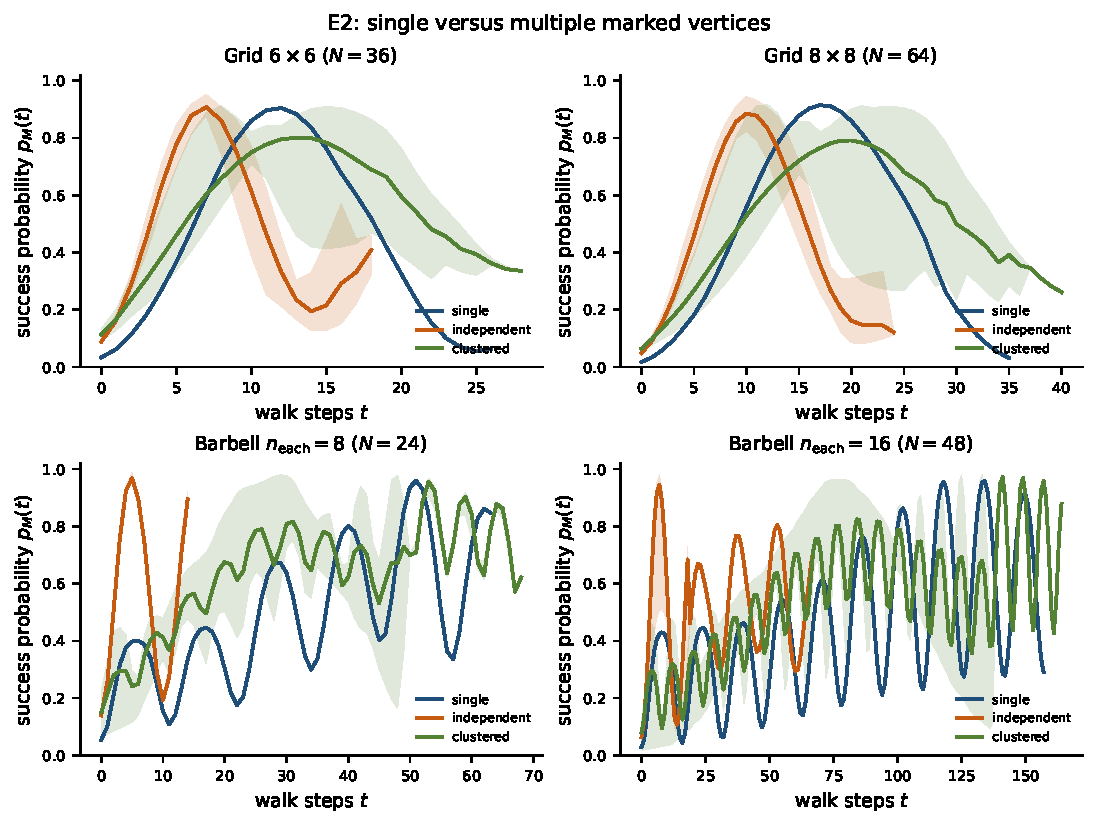
\includegraphics[width=\linewidth]{figures/fig_e2_success.pdf}
  \caption{Success probability versus walk steps for single, independent, and
  clustered marked sets. Shaded bands show the min--max range over three seeds
  (two distinct sets on the $6\times6$ grid and the barbell graphs). Independent targets peak earlier and remain easier; clustered
  targets follow the single-target curve.}
  \label{fig:e2-success}
\end{figure}

\begin{table}[t]
  \centering
  \small
  \begin{tabular}{@{}llcccc@{}}
    \toprule
    Graph & Marked set & mean $\HT$ & mean $\HT^+$ & $\HT^+/\HT$ & mean $T_q$ \\
    \midrule
    Grid $8\times8$ & single & 95.5 & 95.5 & 1.00 & 17.0 \\
    Grid $8\times8$ & independent & 34.7 & 35.3 & 1.02 & 10.7 \\
    Grid $8\times8$ & clustered & 79.5 & 85.3 & 1.07 & 20.3 \\
    Barbell $n=16$ & single & 2558.0 & 2557.9 & 1.00 & 134.0 \\
    Barbell $n=16$ & independent & 16.8 & 25.4 & 1.52 & 7.0 \\
    Barbell $n=16$ & clustered & 2478.6 & 2507.4 & 1.01 & 115.3 \\
    \bottomrule
  \end{tabular}
  \caption{Selected E2 results. Means are over three seeds (0, 1, 2) of farthest-point sampling for the
  independent and clustered configurations; for the $6\times6$ grid and the
  barbell graphs ($n=8,16$) seeds 0 and 2 give the same set, so only two
  distinct sets enter those means.}
  \label{tab:e2}
\end{table}

\Cref{fig:e2-ht} places classical hitting times against extended hitting times.
For the grid and barbell cases the two quantities are close: the largest ratio
is $1.52$ for independent targets on the barbell, where several targets sit in
different communities. The right panel shows the AGJK adversarial torus
construction, where the ratio grows from $5.5$ at $L=18$ to $8.8$ at $L=36$,
consistent with growth but too small a range to establish the asymptotic rate.
This confirms that a large $\HT^+$ penalty is a structural phenomenon: it
requires a particular arrangement of marked vertices, not merely clustering.
For $L=18$ the interpolated walk still reaches $p_{\max}=0.978$ at $t=6$, so the
Conjecture~3 numerical protocol is not slowed down by the large $\HT^+$ value.

\begin{figure}[t]
  \centering
  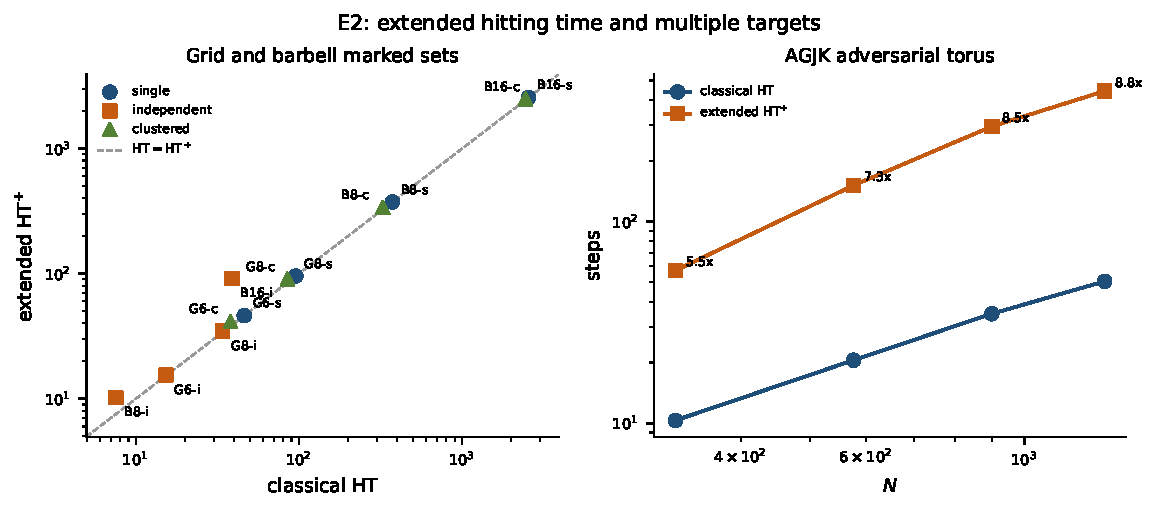
\includegraphics[width=\linewidth]{figures/fig_e2_ht.pdf}
  \caption{Left: classical hitting time versus extended hitting time for the
  grid and barbell marked sets; the dashed line is $\HT=\HT^+$. Right: the AGJK
  adversarial torus construction, where $\HT^+$ grows much faster than $\HT$.
  Labels give the ratio $\HT^+/\HT$.}
  \label{fig:e2-ht}
\end{figure}

\FloatBarrier
\subsection{Semantic activation (E3)}
\label{sec:results-e3}

\Cref{fig:e3} shows the toy semantic graph and the target activation from the
cue \texttt{animal} to two targets: \texttt{dog} (distance $1$) and
\texttt{violin} (distance $4$). The spectral gap is $\lambda_1=0.0333$, giving a
relaxation time of $30.0$ steps. For the near target the CTQW peak is $0.237$ at
$\tau=4.75$, compared with a CRW peak of $0.158$ at $\tau=0.13$. For the far
target the gap is larger: CTQW reaches $0.247$ at $\tau=6.86$, while the CRW
only reaches $0.046$, essentially its stationary value.

\begin{figure}[t]
  \centering
  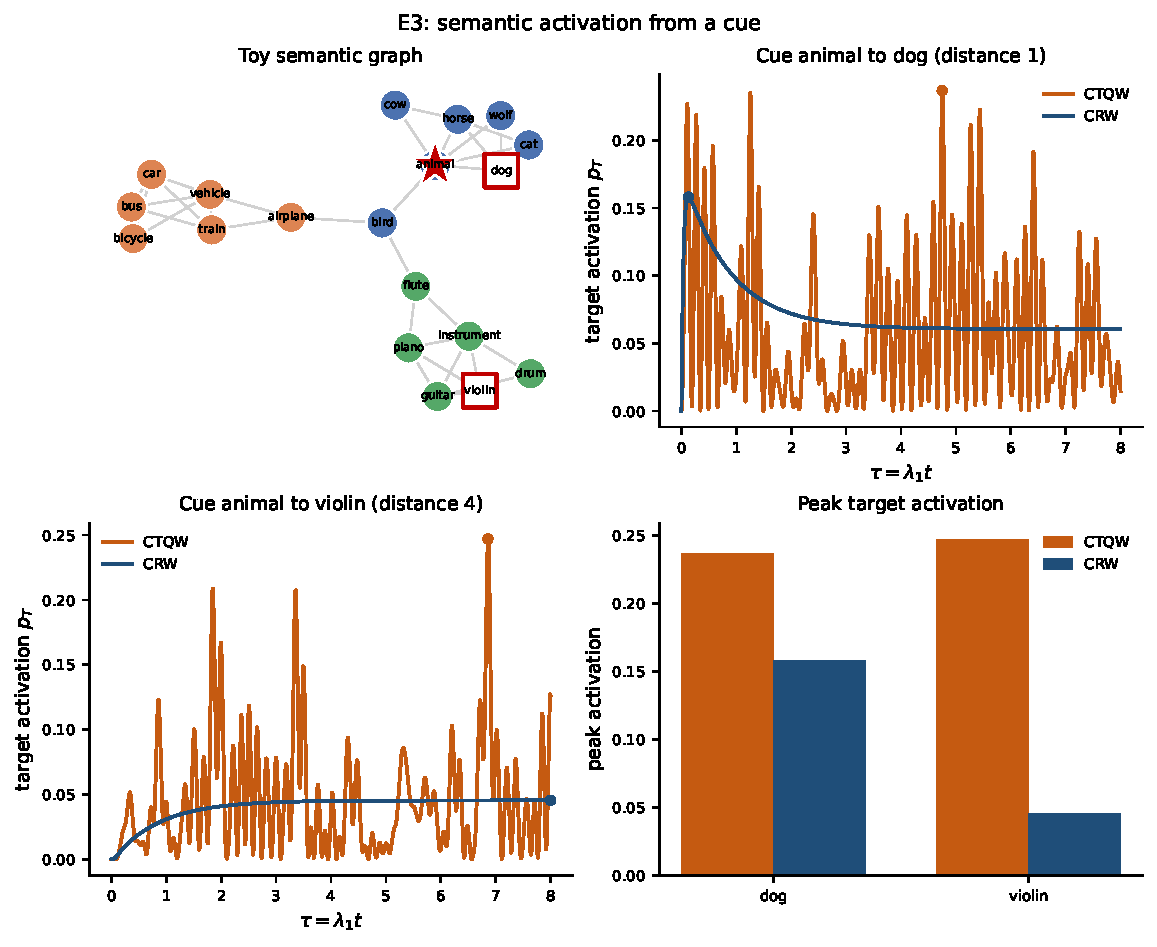
\includegraphics[width=\linewidth]{figures/fig_e3_semantic.pdf}
  \caption{Toy semantic graph and target activation from the cue
  \texttt{animal}. Time is normalized by the spectral gap. The CTQW produces
  larger and later peaks than the CRW, especially for the cross-community
  target \texttt{violin}.}
  \label{fig:e3}
\end{figure}

The activation curves show a clear semantic-distance effect. For the near
target the CRW has a higher area under the curve ($0.580$ versus $0.481$)
because it activates the neighbor immediately and then relaxes. For the far
target the CTQW has a higher AUC ($0.360$ versus $0.324$) and a much higher
peak, while the CRW spreads almost uniformly. The expected radius at the CTQW
peak is also larger ($2.99$ versus $2.36$), indicating that the quantum walk
maintains a broader, more coherent activation pattern instead of collapsing
onto the local neighborhood.

\FloatBarrier
\subsection{Multi-alternative choice under coupling (E4)}
\label{sec:results-e4}

The decision experiment has the same pitfall as E5. Our first readout took
the choice distribution at the first time the total option probability
crossed $0.5$. Because the coherent walk oscillates, that time jumps between
very different phases when the graph changes slightly. Across the laziness
sweep $\eta\in\{0,0.05,0.1,0.2\}$ and ten draws of $\pm20\%$ edge-weight jitter,
the probability of the uncoupled option under this readout moves by a median
of $0.44$ and up to $0.78$ (\cref{fig:e4}, bottom right), so it cannot support
any claim about the effect of coupling. We replace it
with two phase-free quantum readouts: \emph{random stopping}, the choice
distribution averaged over a uniform stopping time $t\in\{1,\dots,400\}$, and
\emph{detection}, in which a position measurement at rate $p=0.2$ per step
ends the decision as soon as it lands on an option terminal.

Under the detection readout the result is stable: the spread is at most
$0.045$, smaller than that of the classical absorbing walk ($0.065$). The
random-stopping readout is in between (median $0.08$, maximum $0.26$).
Both phase-free quantum readouts show the same effect (\cref{fig:e4}): coupling
two options moves probability to the option that is not coupled, and the
shift grows with $c$. Under detection it is monotone in all three graphs;
under random stopping it is monotone up to dips below $0.004$ on the
asymmetric graph. In the symmetric three-option graph the
uncoupled option goes from $1/3$ to $0.499$ at $c=2$ under detection ($0.580$
under random stopping), while the coupled pair falls to $0.250$ each. In the
four-option graph the two uncoupled options together go from $0.500$ to
$0.653$. In the asymmetric ($3$--$4$--$5$) graph the uncoupled short branch
goes from $0.342$ to $0.470$, monotonically.

The classical walk behaves differently. On the symmetric graphs its choice
distribution is exactly uniform for every $c$: coupling only moves probability
between the two coupled branches, which stay symmetric with each other. On the
asymmetric graph coupling mostly redistributes mass inside the coupled pair
(option B rises from $0.32$ to $0.51$, option C falls from $0.26$ to $0.09$) while the uncoupled
option changes little ($0.426$ to $0.409$). The quantum effect is therefore a
qualitative difference, not a matter of degree. Its cost is time: the mean
decision time under detection is $31$--$44$ steps, against $17$--$27$ for the
classical walk, because only one step in five is measured.

\begin{figure}[t]
  \centering
  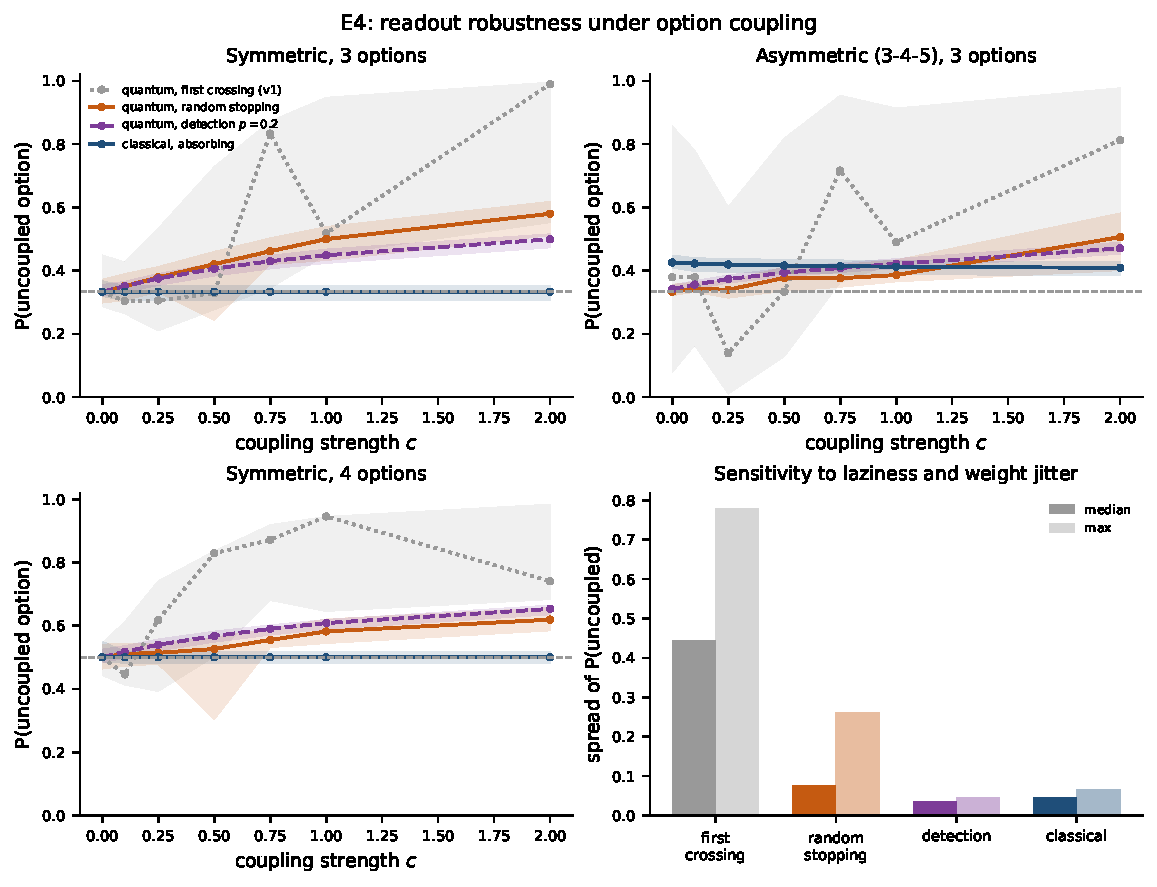
\includegraphics[width=\linewidth]{figures/fig_e4_robustness.pdf}
  \caption{Choice under option coupling. Panels 1--3: probability of the
  uncoupled option(s) versus coupling $c$ for four readouts; lines are the
  nominal graph ($\eta=0.1$), bands span the laziness sweep and edge-weight
  jitter. The dashed grey line is the uniform baseline. Bottom right: spread of
  that probability across variants for each readout.}
  \label{fig:e4}
\end{figure}

This is a model-level analogue of the similarity effect in multi-alternative
choice: when two alternatives become more similar, the dissimilar alternative
gains share. In the walk model it arises from interference between the coupled
branches; the classical walk on the same graph does not produce it.

\FloatBarrier
\subsection{Coherence versus intermediate measurement (E5)}
\label{sec:results-e5}

A pure quantum walk does not approach its target monotonically; its success
probability oscillates. Any comparison at a single deadline therefore depends
on where that deadline falls in the oscillation. The top-left panel of
\cref{fig:e5} makes this explicit for the single-target grid: at $p=0$ the
readout success peaks at $0.449$ at $T=13$ and is only $0.013$ at $T=20$. An
earlier version of this analysis compared measurement rates at $T=20$ only and
reported a $12\times$ gain from measurement; that gain came from the deadline
sitting in a trough. Under the unified lazy walk ($\eta=0.1$), which shifts
the oscillation, the same comparison gives only $1.6\times$, and averaging over
deadlines removes the gain entirely (below). We therefore report two
deadline-free readouts.

\paragraph{Readout model.} Here the observer reads the position once at the
deadline $T$, and intermediate measurements only reset the walk. Averaging the
success over a uniform deadline $T\in\{1,\dots,H\}$ removes the phase
dependence. With $H=120$ the pure walk is best or tied in three of four cases
(grid single $0.042$, grid cluster $0.156$, toy single $0.038$); only the
clustered semantic target gains, from $0.178$ to $0.200$ at $p=0.2$.
Measurement mainly flattens the curve: the coefficient of variation of $p_T$
drops from $1.50$ to $0.37$ on the single-target grid at $p=0.2$. In this
model, measurement buys predictability, not success.

\paragraph{Detection model.} Here a measurement that lands on a marked vertex
ends the search, as in a recognition event, and a final readout is made at the
deadline. Now $p=0$ is the pure walk read once at $T$ and $p=1$ is exactly the
classical first-passage probability $\Pr[\tau_M\le T]$.
\Cref{tab:e5} and the right half of \cref{fig:e5} show the result. Before
$T\approx15$ the pure walk wins in every case, because its first coherent peak
arrives before measurement has had time to help. For clustered targets an
intermediate rate is best for $T\gtrsim20$, apart from single-step revisits of
a later pure-walk peak (e.g.\ $T=35$ on the grid):
$p^\ast=0.2$--$0.3$ finds the cluster by $T=40$ with probability
$0.455$ (grid) and $0.451$ (semantic graph), versus $0.326$ and $0.342$ for the
classical walk and $0.055$ and $0.158$ for the pure walk. By $T=120$ the
advantage over the classical walk is smaller but still present ($0.862$ versus
$0.811$; $0.844$ versus $0.703$). For single targets the optimum moves toward
the classical limit as the deadline grows, though not monotonically: on the
grid $p^\ast$ goes from $0$ (near the first quantum peak) through
$0.2$--$0.5$, with a brief return to $0$ at $T=34$--$36$, to $1$ from $T=71$;
on the semantic graph the classical walk is best for $13\le T\le85$ and within
$0.01$ of the best ($p=0.5$) afterwards.

\begin{figure}[t]
  \centering
  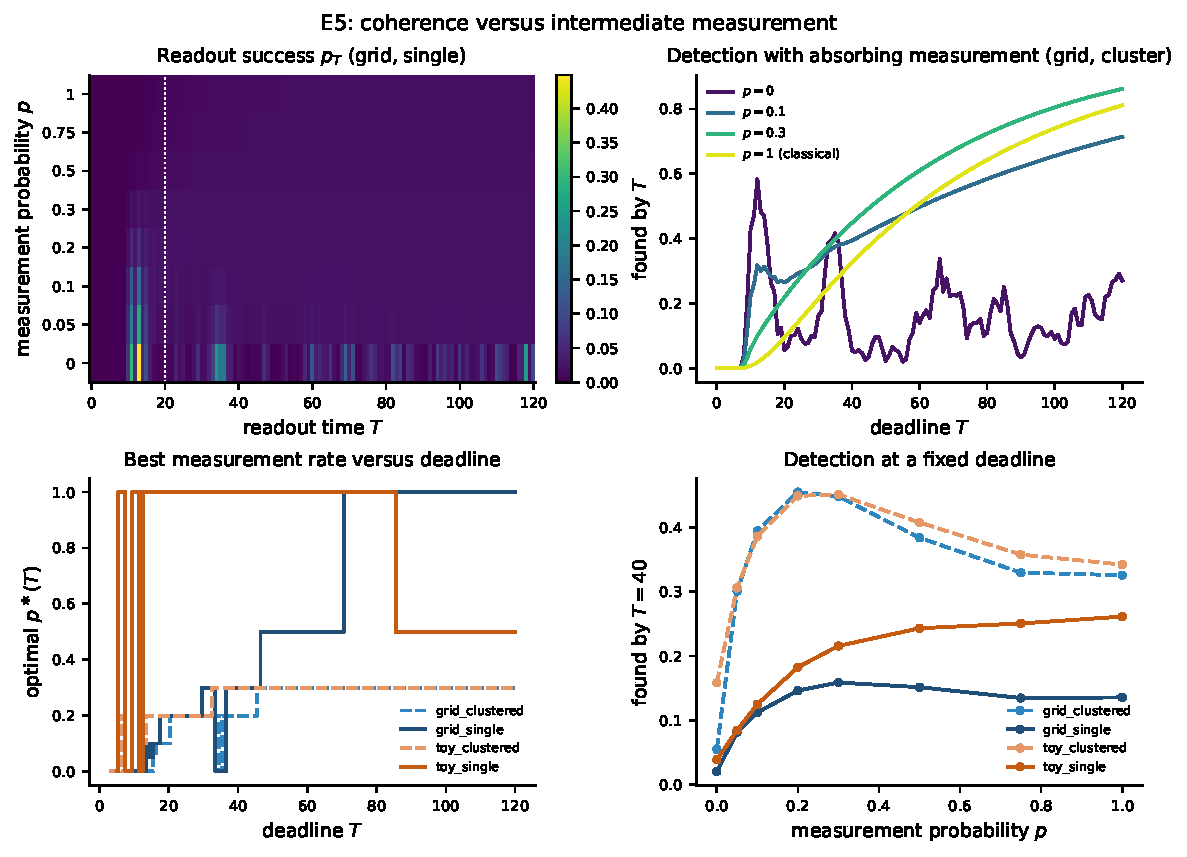
\includegraphics[width=\linewidth]{figures/fig_e5_robustness.pdf}
  \caption{Coherence versus intermediate measurement. Top left: readout
  success $p_T$ on the single-target grid (rows are the tested $p$ values,
  not to scale); the dotted line marks the old deadline $T=20$. Top right: probability that the target cluster has been found
  by $T$ in the detection model. Bottom left: best measurement rate $p^\ast$ as
  a function of the deadline. Bottom right: detection probability at $T=40$
  versus $p$.}
  \label{fig:e5}
\end{figure}

\begin{table}[t]
  \centering
  \small
  \begin{tabular}{@{}lccccc@{}}
    \toprule
    & \multicolumn{2}{c}{pure walk ($p=0$)}
    & \multicolumn{3}{c}{found by $T=40$ (detection model)} \\
    \cmidrule(lr){2-3}\cmidrule(l){4-6}
    Case & peak & at $t$ & $p=0$ & $p=1$ & best $p$ (value) \\
    \midrule
    Grid, single & 0.449 & 13 & 0.020 & 0.136 & 0.3 (0.159) \\
    Grid, clustered & 0.583 & 12 & 0.055 & 0.326 & 0.2 (0.455) \\
    Toy, single & 0.198 & 107 & 0.039 & 0.261 & 1.0 (0.261) \\
    Toy, clustered & 0.394 & 58 & 0.158 & 0.342 & 0.3 (0.451) \\
    \bottomrule
  \end{tabular}
  \caption{E5 summary. The pure walk has the highest peak in every case but
  needs that peak to be timed; with absorbing measurement an intermediate rate
  beats both limits for clustered targets.}
  \label{tab:e5}
\end{table}

The picture is a three-way tradeoff. A perfectly timed coherent search has the
highest peak, the classical walk accumulates detections reliably, and a
partially coherent search combines fast spreading with the ability to stop
once the target is seen. The last option wins when the target is extended
(a cluster of related concepts) and the deadline is moderate.

\FloatBarrier
\subsection{Summary of empirical findings}
\label{sec:results-summary}

The experiments support three conclusions. First, the quantum search time
tracks $\sqrt{\HT}$ across the synthetic families, and independent targets are
easier than clustered ones. Second, a large $\HT^+/\HT$ gap is a structural
effect of the marked-set arrangement, not a generic consequence of having
multiple targets. Third, the cognitive layer is sensitive to graph structure:
semantic distance changes activation timing, option coupling shifts quantum
choice toward the uncoupled option while leaving the classical choice
unchanged, and when a measurement can end the search, an intermediate
measurement rate finds clustered targets faster than either the pure quantum
or the classical walk, even though the pure walk keeps the highest timed peak.
